\chapter{Theory}
\label{chap:theory}

\section{The standard model of particle physics}
\begin{itemize}
    \item Lagrangian formalism. Smooth transition to EFT.
    \item Asymptotic freedom: jets
\end{itemize}

\section{Higgs boson phenomenology}
Different production mechanisms. ttH, tH as means for measuring the top yukawa directly, ggH is indirect. Higgs self coupling. Throughout, no distinction between quark and antiquark.

\section{Simplified template cross sections}\label{sec:theory_stxs}
qqH definition. ggZH had grouping with ggH. Define: Truth-level (consider changing to particle level) vs Reco-level. Jet definition. Drop GeV in definitions throughout. Cite STXS.

\begin{landscape}
\begin{figure}[htbp]
  \centering
  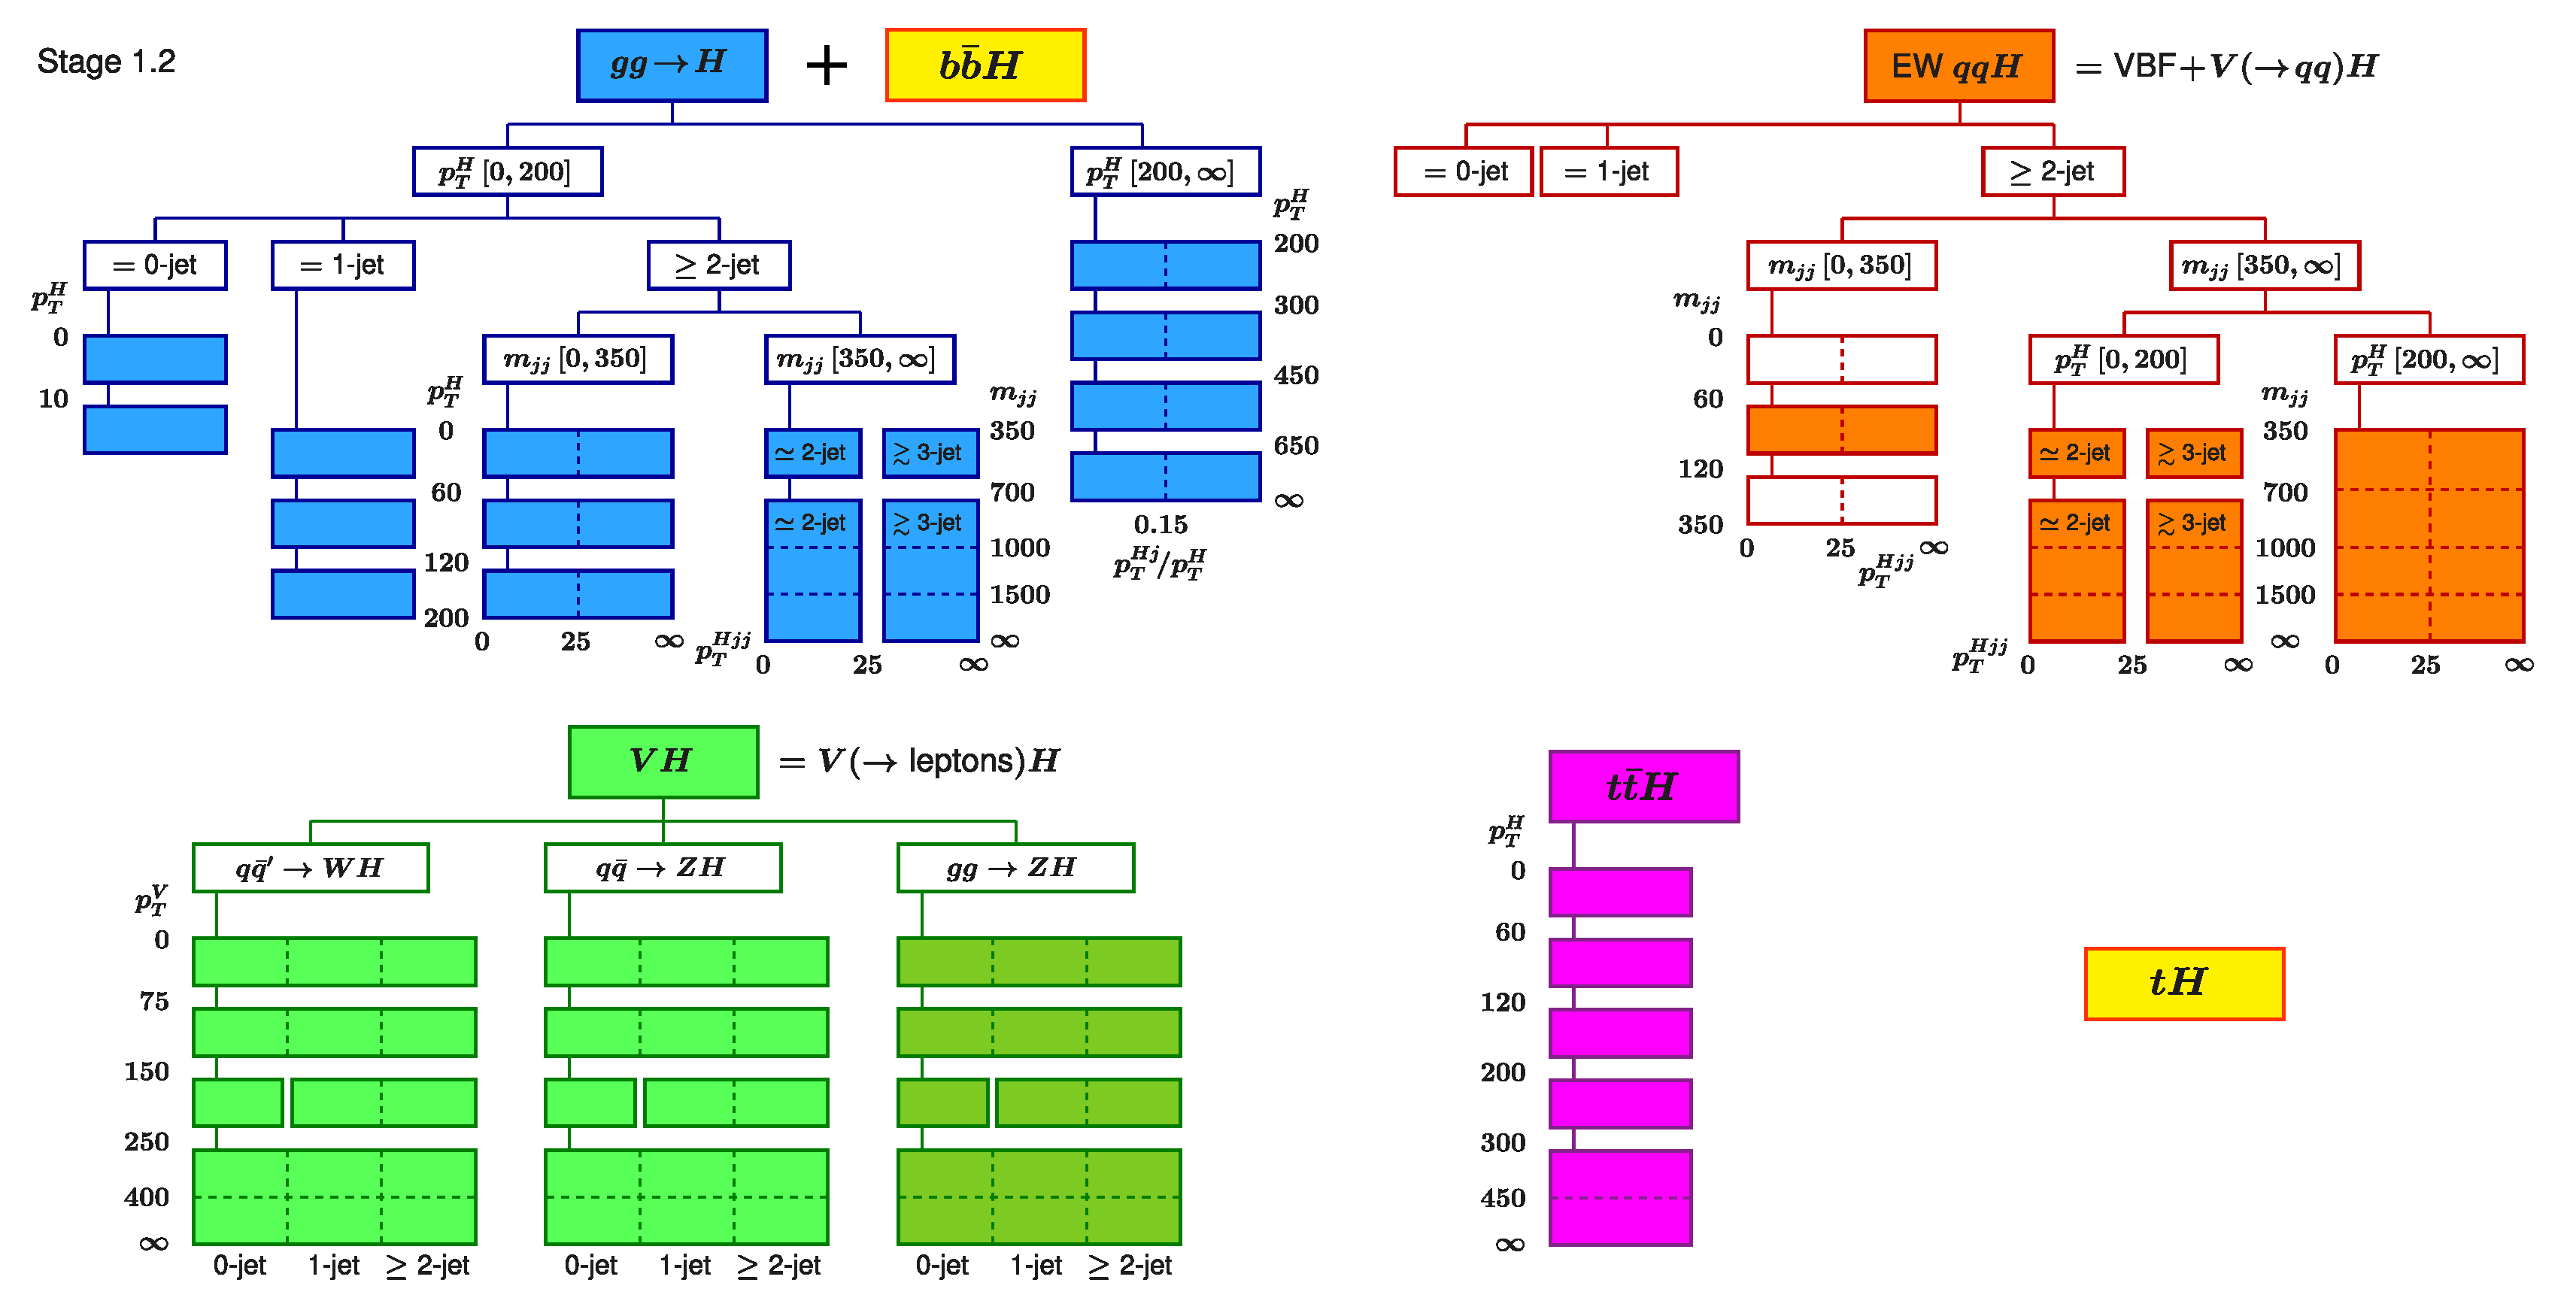
\includegraphics[width=1\linewidth]{Figures/theory/stxs_schematic.pdf}
  \caption[STXS stage 1.2 binning scheme]
  {
    A schematic showing the complete STXS stage 1.2 binning scheme. The solid lines define each stage 1.2 bin. The ggH region (blue) is split into bins using the Higgs boson transverse momentum, \ptH, the number of jets, and an additional VBF-like region with high dijet invariant mass, \mjj. The VBF and VH hadronic production modes are considered together as EW qqH production (orange). The bins here are deined using \ptH, the number of jets, \mjj, and the transverse momentum of the Higgs boson plus dijet system, \ptHjj, in the VBF-like region. The VH leptonic bins (green) are defined by the number of jets and the transverse momentum of the vector boson, \ptV. The ttH production mode (magenta) is split only by \ptH. Finally, the tH and bbH processes (yellow) are not further divided at STXS stage 1.2. In this analysis, bbH is grouped with the definition of ggH.
  }
  \label{fig:stxs_schematic}
\end{figure}
\end{landscape}


\begin{table}[htb!]
    \caption[ggH STXS stage 1.2 definitions and fractions]{Make clear definitions of jets etc  distance param}
    \label{tab:ggH_definitions}
    % \vspace{.5cm}
    \centering
    \scriptsize
    \renewcommand{\arraystretch}{1.2}
    \setlength{\tabcolsep}{5pt}
    \hspace*{-5cm}
    \begin{tabular}{l|cccc}
   \multirow{2}{*}{STXS bin} & \multirow{2}{*}{\begin{tabular}[c]{@{}c@{}}Definition\\ units of $\ptH$, $\mjj$ and $\ptHjj$ in GeV\end{tabular}} & \multicolumn{2}{c}{Fraction of cross section} & \multirow{2}{*}{$\sigma_{\text{SM}}\mathcal{B}$~(fb)} \\
    &  & ggH & gg $\rightarrow$ Z(q$\bar{\rm{q}}$)H &  \\ [\cmsTabSkip] \hline
   ggH forward & $|Y_H| > 2.5$ & 8.09\% & 2.73\% & 8.93 \\ [\cmsTabSkip]
   ggH 0J low $\ptH$ & Exactly 0 jets, $\ptH$~$<$~10 & 13.87\% & 0.01\% & 15.30 \\
   ggH 0J high $\ptH$ & Exactly 0 jets, 10~$<$~$\ptH$~$<$~200 & 39.40\% & 0.29\% & 43.45 \\ [\cmsTabSkip]
   ggH 1J low $\ptH$ & Exactly 1 jet, $\ptH$~$<$~60 & 14.77\% & 2.00\% & 16.29 \\
   ggH 1J med $\ptH$ & Exactly 1 jet, 60~$<$~$\ptH$~$<$~120 & 10.23\% & 5.34\% & 11.29 \\
   ggH 1J high $\ptH$ & Exactly 1 jet, 120~$<$~$\ptH$~$<$~200 & 1.82\% & 3.53\% & 2.01 \\  [\cmsTabSkip]
   ggH $\geq$2J low $\ptH$ & At least 2 jets, $\ptH$~$<$~60, $\mjj$~$<$~350 & 2.56\% & 5.74\% & 2.83 \\
   ggH $\geq$2J med $\ptH$ & At least 2 jets, 60~$<$~$\ptH$~$<$~120, $\mjj$~$<$~350 & 4.10\% & 19.63\% & 4.56 \\
   ggH $\geq$2J high $\ptH$ & At least 2 jets, 120~$<$~$\ptH$~$<$~200, $\mjj$~$<$~350 & 1.88\% & 29.55\% & 2.13 \\  [\cmsTabSkip]
   ggH BSM 200~$<$~$\ptH$~$<$~300 & No jet requirements, 200~$<$~$\ptH$~$<$~300 & 0.98\% & 13.93\% & 1.11 \\
   ggH BSM 300~$<$~$\ptH$~$<$~450 & No jet requirements, 300~$<$~$\ptH$~$<$~450 & 0.25\% & 3.86\% & 0.28 \\
   ggH BSM 450~$<$~$\ptH$~$<$~650 & No jet requirements, 450~$<$~$\ptH$~$<$~650 & 0.03\% & 0.77\% & 0.03 \\
   ggH BSM $\ptH$~$>$~650 & No jet requirements, $\ptH$~$>$~650 & 0.01\% & 0.20\% & 0.01 \\ [\cmsTabSkip]
   ggH VBF-like low $\mjj$ low $\ptHjj$ & \begin{tabular}[c]{@{}c@{}}At least 2 jets, $\ptH$~$<$~200,\\ 350~$<$~$\mjj$~$<$~700, $\ptHjj$~$<$~25\end{tabular} & 0.63\% & 1.14\% & 0.70 \\
   ggH VBF-like low $\mjj$ high $\ptHjj$ & \begin{tabular}[c]{@{}c@{}}At least 2 jets, $\ptH$~$<$~200,\\ 350~$<$~$\mjj$~$<$~700, $\ptHjj$~$>$~25\end{tabular} & 0.77\% & 8.06\% & 0.86 \\
   ggH VBF-like high $\mjj$ low $\ptHjj$ & \begin{tabular}[c]{@{}c@{}}At least 2 jets, $\ptH$~$<$~200,\\ $\mjj$~$>$~700, $\ptHjj$~$<$~25\end{tabular} & 0.28\% & 0.36\% & 0.31 \\
   ggH VBF-like high $\mjj$ high $\ptHjj$ & \begin{tabular}[c]{@{}c@{}}At least 2 jets, $\ptH$~$<$~200,\\ $\mjj$~$>$~700, $\ptHjj$~$>$~25\end{tabular} & 0.32\% & 2.85\% & 0.36 \\
\end{tabular}
    \hspace*{-5cm}
\end{table}

\begin{table}[htb!]
    \caption[qqH STXS stage 1.2 definitions and fractions]{Make clear definitions of jets etc distance param}
    \label{tab:qqH_definitions}
    % \vspace{.5cm}
    \centering
    \scriptsize
    \renewcommand{\arraystretch}{1.2}
    \setlength{\tabcolsep}{5pt}
    \hspace*{-5cm}
    \begin{tabular}{l|c|ccc|c}
   \multirow{2}{*}{STXS bin} & \multirow{2}{*}{\begin{tabular}[c]{@{}c@{}}Definition\\ units of $p_T^H$, $\mjj$ and $\ptHjj$ in GeV\end{tabular}} & \multicolumn{3}{c|}{Fraction of total} & \multirow{2}{*}{$\sigma_{\text{SM}}\mathcal{B}$~[fb]} \\ 
    &  & VBF & qq$\rightarrow$W(qq)H & qq$\rightarrow$Z(qq)H &  \\ [\cmsTabSkip] \hline
   qqH forward & $|Y_H| > 2.5$ & 6.69\% & 12.57\% & 9.84\% & 0.98 \\ [\cmsTabSkip]
   %\multicolumn{6}{c}{$|Y_H| < 2.5$} \\ \hline
   qqH 0J & Exactly 0 jets & 6.95\% & 5.70\% & 3.73\% & 0.77 \\ 
   qqH 1J & Exactly 1 jet & 32.83\% & 31.13\% & 25.03\% & 3.82 \\ 
   qqH $\mjj$~$<$~60 & At least 2 jets, $\mjj$~$<$~60 & 1.36\% & 3.58\% & 2.72\% & 0.23 \\ 
   qqH VH-like & At least 2 jets, 60~$<$~$\mjj$~$<$~120 & 2.40\% & 29.43\% & 28.94\% & 1.23 \\ 
   qqH 120~$<$~$\mjj$~$<$~350 & At least 2 jets, 120~$<$~$\mjj$~$<$~350 & 12.34\% & 13.92\% & 12.59\% & 1.53 \\ [\cmsTabSkip]
   qqH VBF-like low $\mjj$ low $\ptHjj$ & \begin{tabular}[c]{@{}c@{}}At least 2 jets, $\ptH$~$<$~200,\\ 350~$<$~$\mjj$~$<$~700, $\ptHjj$~$<$~25\end{tabular} & 10.26\% & 0.44\% & 0.35\% & 0.90 \\ 
   qqH VBF-like low $\mjj$ high $\ptHjj$ & \begin{tabular}[c]{@{}c@{}}At least 2 jets, $\ptH$~$<$~200,\\ 350~$<$~$\mjj$~$<$~700, $\ptHjj$~$>$~25\end{tabular} & 3.85\% & 1.86\% & 1.74\% & 0.39 \\ 
   qqH VBF-like high $\mjj$ low $\ptHjj$ & \begin{tabular}[c]{@{}c@{}}At least 2 jets, $\ptH$~$<$~200,\\ $\mjj$~$>$~700, $\ptHjj$~$<$~25\end{tabular} & 15.09\% & 0.09\% & 0.08\% & 1.30 \\ 
   qqH VBF-like high $\mjj$ high $\ptHjj$ & \begin{tabular}[c]{@{}c@{}}At least 2 jets, $\ptH$~$<$~200,\\ $\mjj$~$>$~700, $\ptHjj$~$>$~25\end{tabular} & 4.25\% & 0.40\% & 0.39\% & 0.38 \\ 
   qqH BSM & At least 2 jets, $\mjj$~$>$~350, $p_T^H$~$>$~200 & 3.98\% & 0.88\% & 0.71\% & 0.37 \\ 
\end{tabular}

    \hspace*{-5cm}
\end{table}

\begin{table}[htb!]
    \caption[VH leptonic STXS stage 1.2 definitions and fractions]{Make clear definitions of jets etc}
    \label{tab:vh_definitions}
    % \vspace{.5cm}
    \centering
    \scriptsize
    \renewcommand{\arraystretch}{1.2}
    \setlength{\tabcolsep}{5pt}
    \hspace*{-5cm}
    \begin{tabular}{l|ccccc}
    \hline
   \multirow{2}{*}{STXS bin} & \multirow{2}{*}{\begin{tabular}[c]{@{}c@{}}Definition\\ units of $\ptV$ in GeV\end{tabular}} & \multicolumn{3}{c}{Fraction of cross section} & \multirow{2}{*}{$\sigma_{\text{SM}}\mathcal{B}$~(fb)} \\
    &  & q$\bar{\rm{q}}'\rightarrow$WH & q$\bar{\rm{q}}'\rightarrow$ZH & gg$\rightarrow$ZH &  \\ [\cmsTabSkip] \hline
   WH lep forward& \multirow{3}{*}{$|Y_H| > 2.5$}& 12.13\%& -& -& 0.123 \\
   ZH lep forward& & -& 11.21\%& -& 0.058 \\
   ggZH lep forward& & -& -& 2.71\%& 0.002 \\ [\cmsTabSkip]
   %\multicolumn{6}{c}{$|Y_H| < 2.5$} \\ \hline
   WH lep $\ptV$~$<$~75 & No jet requirements, $\ptV$~$<$~75 & 46.55\% & - & - & 0.473 \\
   WH lep 75~$<$~$\ptV$~$<$~150 & No jet requirements, 75~$<$~$\ptV$~$<$~150 & 29.30\% & - & - & 0.298 \\
   WH lep 0J 150~$<$~$\ptV$~$<$~250 & Exactly 0 jets, 150~$<$~$\ptV$~$<$~250 & 5.10\% & - & - & 0.052 \\
   WH lep $\geq$1J 150~$<$~$\ptV$~$<$~250 & At least 1 jet, 150~$<$~$\ptV$~$<$~250 & 3.97\% & - & - & 0.040 \\
   WH lep $\ptV$~$>$~250 & No jet requirements, $\ptV$~$>$~250 & 2.95\% & - & - & 0.030 \\ [\cmsTabSkip]
   ZH lep $\ptV$~$<$~75 & No jet requirements, $\ptV$~$<$~75 & - & 45.65\% & - & 0.237 \\
   ZH lep 75~$<$~$\ptV$~$<$~150 & No jet requirements, 75~$<$~$\ptV$~$<$~150 & - & 30.70\% & - & 0.160 \\
   ZH lep 0J 150~$<$~$\ptV$~$<$~250 & Exactly 0 jets, 150~$<$~$\ptV$~$<$~250 & - & 5.16\% & - & 0.027 \\
   ZH lep $\geq$1J 150~$<$~$\ptV$~$<$~250 & At least 1 jet, 150~$<$~$\ptV$~$<$~250 & - & 4.27\% & - & 0.022 \\
   ZH lep $\ptV$~$>$~250 & No jet requirements, $\ptV$~$>$~250 & - & 3.01\% & - & 0.016 \\ [\cmsTabSkip]
   ggZH lep $\ptV$~$<$~75 & No jet requirements, $\ptV$~$<$~75 & - & - & 15.96\% & 0.013 \\
   ggZH lep 75~$<$~$\ptV$~$<$~150 & No jet requirements, 75~$<$~$\ptV$~$<$~150 & - & - & 43.32\% & 0.036 \\
   ggZH lep 0J 150~$<$~$\ptV$~$<$~250 & Exactly 0 jets, 150~$<$~$\ptV$~$<$~250 & - & - & 9.08\% & 0.008 \\
   ggZH lep $\geq$1J 150~$<$~$\ptV$~$<$~250 & At least 1 jet, 150~$<$~$\ptV$~$<$~250 & - & - & 20.49\% & 0.017 \\
   ggZH lep $\ptV$~$>$~250 & No jet requirements, $\ptV$~$>$~250 & - & - & 8.45\% & 0.007 \\
   \hline
\end{tabular}

    \hspace*{-5cm}
\end{table}

\begin{table}[htb!]
    \caption[Top-associated and bbH STXS stage 1.2 definitions and fractions]{Make clear definitions of jets etc}
    \label{tab:top_definitions}
    % \vspace{.5cm}
    \centering
    \scriptsize
    \renewcommand{\arraystretch}{1.5}
    \setlength{\tabcolsep}{5pt}
    \hspace*{-5cm}
    \begin{tabular}{l|c|cccc|c}
   \multirow{2}{*}{STXS region} & \multirow{2}{*}{\begin{tabular}[c]{@{}c@{}}Definition\\ units of $\ptH$ in GeV\end{tabular}} & \multicolumn{4}{c|}{Fraction of total} & \multirow{2}{*}{$\sigma_{\text{SM}}\mathcal{B}$~[fb]} \\ 
    &  & ttH & tHq & tHW & bbH &  \\ [\cmsTabSkip] \hline
   ttH forward& \multirow{3}{*}{$|Y_H| > 2.5$}& 1.35\%& -& -& -& 0.016 \\  
   tH forward& & -& 2.79\%& 1.06\%& -& 0.005 \\  
   bbH forward& & -& -& -& 4.87\%& 0.054 \\ [\cmsTabSkip] 
   %\multicolumn{7}{c}{$|Y_H| < 2.5$} \\ \hline
   ttH $\ptH$~$<$~60 & No jet requirements, $\ptH$~$<$~60 & 22.42\% & - & - & - & 0.259 \\ 
   ttH 60~$<$~$\ptH$~$<$~120 & No jet requirements, 60~$<$~$\ptH$~$<$~120 & 34.61\% & - & - & - & 0.400 \\ 
   ttH 120~$<$~$\ptH$~$<$~200 & No jet requirements, 120~$<$~$\ptH$~$<$~200 & 25.60\% & - & - & - & 0.296 \\ 
   ttH 200~$<$~$\ptH$~$<$~300 & No jet requirements, 200~$<$~$\ptH$~$<$~300 & 10.72\% & - & - & - & 0.124 \\ 
   ttH $\ptH$~$>$~300 & No jet requirements, $\ptH$~$>$~300 & 5.31\% & - & - & - & 0.061 \\ [\cmsTabSkip] 
   tH & No additional requirements & - & 97.21\% & 98.94\% & - & 0.204 \\ 
   bbH & No additional requirements & - & - & - & 95.13\% & 1.054 \\ 
\end{tabular}

    \hspace*{-5cm}
\end{table}

\section{Recent Higgs boson results}

\section{Effective field theory}\label{sec:theory_eft}

UV & IR. Replace non-local interactions via exchange of new particles by contact interactions, expressed using higher dimensional operators. This restricts validity of EFT to be below a certain energy scale. Replace below with expansion for all orders.

\begin{equation}\label{eq:eft_expansion}
    \mathcal{L}_{\rm{EFT}} = \mathcal{L}_{\rm{SM}} + \sum^{N_{\rm{dim6}}}_p \frac{w^{(6)}_p}{\Lambda^2}\mathcal{O}^{(6)}_p + \sum^{N_{\rm{dim8}}}_p \frac{w^{(8)}_p}{\Lambda^4}\mathcal{O}^{(8)}_p + ... ,
\end{equation}

\subsection{EFT basis}
\begin{itemize}
    \item HEFT vs SMEFT
    \item Full EFT extension, only consider dim-6 in this thesis (motivations)
    \item Definition of a basis: complete and non-redundant set of operators.
    \item Lagrangian and then effect on matrix element: SM + interference + BSM. A comment on dim-8.
    \item Match EFT constraints to constrain masses and couplings in UV complete BSM theories
    \item Briefly discuss HEL and SMEFTsim: save intricate details for Chapter 7
\end{itemize}